\exer{Implémentation des graphes par une matrice d'adjacence}


On considère le graphe \texttt{G} suivant, où le nombre situé sur l'arête joignant deux sommets est leur distance, supposée entière. 

\begin{center}
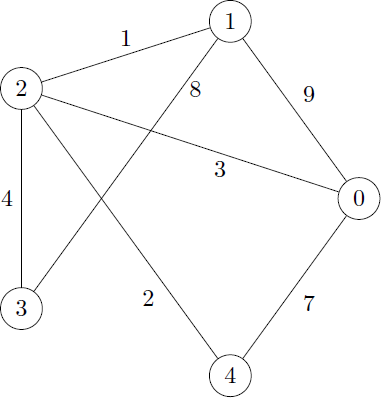
\includegraphics[width=7cm]{images/application_matrice}
\end{center}


\question{Construire la matrice $\left( G_{ij}\right)_{0\leq i,j\leq 4}$, matrice de distances du graphe \texttt{G}, définie par :
<< pour tous les indices $i$, $j$, $G_{ij}$ représente la distance entre les sommets $i$ et $j$,
ou encore la longueur de l'arête reliant les sommets $i$ et~$j$~>>. Cette matrice sera implémentée sous forme d'une liste de listes. (Chaque << sous-liste >> représentant une ligne de la matrice d'adjacence. 
On convient que, lorsque les sommets ne sont pas reliés, cette distance vaut $-1$. La distance du
sommet $i$ à lui-même est égale à 0.}


%\question{Écrire une suite d'instructions permettant de dresser à partir de la matrice \texttt{M} la liste des voisins du sommet 4.}

\question{Écrire une fonction \texttt{voisins(G:list, i:int) -> list}, d'argument la matrice d'adjacence \texttt{G} et un sommet $i$, renvoyant la liste des voisins du sommet~$i$.}


\question{Écrire une fonction \texttt{arretes(G:list) -> list}, renvoyant la liste des arêtes. Les arêtes seront constitués de couples de sommets (l'arête entre les sommets 0 et 1 sera donnée par \texttt{(0,1)}.}

Les instructions suivantes permettent de tracer un graphe. 

\begin{lstlisting}
import networkx as nx

def plot_graphe(G):
    Gx = nx.Graph()
    edges = arretes(G)
    Gx.add_edges_from(edges)
    nx.draw(Gx,with_labels = True)
    plt.show()
plot_graphe(M)
\end{lstlisting}

\question{Écrire et tester la fonction \texttt{plot\_graphe(G)}.}

\question{Écrire une fonction \texttt{degre(G:list, i:int) -> int}, d'argument un sommet $i$, renvoyant le nombre des voisins du sommet $i$, c'est-à-dire le nombre d’arêtes issues de $i$.}


\question{Écrire une fonction \texttt{longueur(G:list,L:list) -> int}, d’argument une liste \texttt{L} de sommets de \texttt{G}, renvoyant la longueur du trajet d'écrit par cette liste \texttt{L}, c’est-à-dire la somme des longueurs des arêtes empruntées. Si le trajet n'est pas possible, la fonction renverra $-1$.}

\question{Écrire la fonction \texttt{ajout\_sommet(G:list, L:list, poids : list) -> None} permettant d'ajouter un sommet au graphe. \texttt{L} désigne la liste des sommets auxquels le nouveau sommet est relié, \texttt{poids} la liste des poids respectifs. \texttt{ajout\_sommet} agit avec effet de bord sur \texttt{G}.}

\question{Écrire la fonction \texttt{supprime\_sommet(G:list, i: int) -> None} permettant de supprimer le sommet $i$ du graphe.}
%
%
%\subsubsection*{Implémentation d'un graphe par une liste d'adjacence}
%Pour implémenter le graphe, on utilise une liste \texttt{G} qui a pour taille le nombre de sommets. Chaque élément \texttt{G[i]} est la liste des voisins de \texttt{i}. 
%
%On s'intéresse au graphe précédent, \textbf{sans les pondérations}.  Dans ce cas, \texttt{G[0]=[1,2,4]} car Les sommets 1, 2 et 4 sont des voisins de 0.
%
%\question{Construire la liste d'adjacence \texttt{G} en utilisant la méthode énoncée ci-dessus.}
%
%\question{Écrire une fonction \texttt{voisins\_l(G:list, i:int) -> list}, d'argument la liste d'adjacence \texttt{G} et un sommet $i$, renvoyant la liste des voisins du sommet~$i$.}
%
%\question{Écrire une fonction \texttt{degre\_l(G:list, i:int) -> int}, d'argument un sommet $i$, renvoyant le nombre des voisins du sommet $i$, c'est-à-dire le nombre d’arêtes issues de $i$.}
%
%\question{Écrire la fonction \texttt{ajout\_sommet\_l(G:list, L:list) -> None} permettant d'ajouter un sommet au graphe. Cette fonction prendra comme argument \texttt{G} liste d'adjacence du graphe et \texttt{L} la liste des sommets auxquels le nouveau sommet est relié. \texttt{ajout\_sommet} agit avec effet de bord sur \texttt{G}.}
%
%\question{Écrire la fonction \texttt{supprime\_sommet\_l(G:list, i: int) -> None} permettant de supprimer le sommet $i$ du graphe.}
